% Allgemeines Dokumentenformnat
\documentclass[a4paper,11pt,headsepline,hidelinks]{scrartcl}
\usepackage{acronym}
\usepackage{comment}
\usepackage[table, xcdraw]{xcolor}
\usepackage[
automark, % Kapitelangaben in Kopfzeile automatisch erstellen
headsepline, % Trennlinie unter Kopfzeile
ilines % Trennlinie linksbündig ausrichten
]{scrlayer-scrpage}
% Kopf- und Fußzeilen ----------------------------------------------------------
\pagestyle{scrheadings}
% chapterpagestyle gibt es nicht in scrartcl
%\renewcommand{\chapterpagestyle}{scrheadings}
\clearscrheadfoot

% Kopfzeile 
\renewcommand{\headfont}{\normalfont} % Schriftform der Kopfzeile
%\ihead{\large{\textsc{Anwendung zur Erfassung und Bearbeitung von\\ umfangreichen Anwender-Softwaretests}}\\ \small{Softwaretest Manager} \\[0ex]}
%\chead{}
\ohead{
\includegraphics[scale=0.2]{bilder/k&m.png}}
%\setlength{\headheight}{15mm} % Höhe der Kopfzeile
%\setheadwidth[0pt]{textwithmarginpar} % Kopfzeile über den Text hinaus verbreitern (falls Logo den Text überdeckt)

% Fußzeile
\ifoot{Jakob Schumann}
\cfoot{}
\ofoot{\pagemark}

% Überschriften nach DIN 5008 in einer Fluchtlinie
% ------------------------------------------------------------------------------

% Abstand zwischen Nummerierung und Überschrift definieren
% > Schön wäre hier die dynamische Berechnung des Abstandes in Abhängigkeit
% > der Verschachtelungstiefe des Inhaltsverzeichnisses
\newcommand{\headingSpace}{1.5cm}

% Abschnittsüberschriften im selben Stil wie beim Inhaltsverzeichnis einrücken
\renewcommand*{\othersectionlevelsformat}[3]{
	\makebox[\headingSpace][l]{#3\autodot}
}

% Für die Einrückung wird das Paket tocloft benötigt
%\cftsetindents{chapter}{0.0cm}{\headingSpace}
%\cftsetindents{section}{0.0cm}{\headingSpace}
%\cftsetindents{subsection}{0.0cm}{\headingSpace}
%\cftsetindents{subsubsection}{0.0cm}{\headingSpace}
%\cftsetindents{figure}{0.0cm}{\headingSpace}
%\cftsetindents{table}{0.0cm}{\headingSpace}
% Weitere Pakete
% Grafiken
\usepackage{graphicx}
\usepackage{float}

% Deutsche Sonderzeichen
 %\usepackage{ngerman}

% Deutsche Silbentrennung
\usepackage[ngerman]{babel} 

% Eurozeichen einbinden
\usepackage[right]{eurosym} 

% Umlaute in UTF8
\usepackage[utf8]{inputenc}

% Zeichencodierung
\usepackage[T1]{fontenc}
\usepackage{mathptmx}
\usepackage{helvet} 
%\usepackage{fix-cm}
%\newcommand{\changefont}[3]{	\fontfamily{#1} \fontseries{#2} \fontshape{#3} \selectfont}
%\changefont{ptm}{m}{sl}

% mehrseitige Tabellen
\usepackage{longtable}

% Seitenränder
\usepackage{geometry}
\geometry{left=2.5cm, right=2cm, top=4cm, bottom=2cm}

% Boxen im Text
\usepackage{fancybox}

% schöne URLs
\usepackage[hyphens,obeyspaces,spaces]{url} % schöne URLs

% Textfarben
\usepackage{color}

% Mathematische Symbole
\usepackage{amssymb}

% Inhaltsverzeichnis + Querverweiss
\usepackage[bookmarksnumbered,pdftitle={Abschlussprojektdokumentation},hyperfootnotes=false]{hyperref}

\hypersetup{
	colorlinks=false,
	linkcolor=blue,
	filecolor=magenta,
	urlcolor=cyan,
}

% Kopfzeile
%\usepackage{fancyhdr}
%\pagestyle{fancy}
%\fancyhf{}
%\fancyhead[L]{\nouppercase{\leftmark}}
%\fancyhead[C]{}
%\fancyhead[R]{\thepage}
%\renewcommand{\headrulewidth}{0.4pt}

% Tabellen allgemein
\usepackage{array}

% Zitierweise
\bibliographystyle{alphadin}

% Kein Zwischenraum nach Satzzeichen
\frenchspacing

% Zeilenabstand
\usepackage{setspace}
\usepackage{parskip}
\parskip 6pt plus 3pt minus 1pt

% Bildzeichner
\usepackage{capt-of}
\usepackage{caption}

% Stichwortverzeichnis
\usepackage{makeidx}
%\usepackage{unnumberedtotoc}

% Aufzählungen
\usepackage{listings}
\lstset{numbers=left, numberstyle=\tiny, numbersep=5pt, keywordstyle=\color{black}\bfseries, stringstyle=\ttfamily,showstringspaces=false,basicstyle=\footnotesize,captionpos=b}
\lstset{language=bash}

% Indexerstellubg
\makeindex

% Glossar
\usepackage{glossaries}
\makeglossaries
\newglossaryentry{k8s}{name={Kubernetes}, description={Orchestrator für Containeranwendungen}, text={\underline{Kubernetes}}}
\newglossaryentry{vue}{name={Vue.js}, description={Ein clientseitiges Javascript-Framework nach dem Model-View-ViewModel-Entwurfsmuster für das Erstellen von Webanwendungen}, text={\underline{Vue.js}}}
\newglossaryentry{vuetify}{name={Vuetify}, description={Eine Vue.js Oberflächenkomponentenbibliothek}, text={\underline{Vuetify}}}
\newglossaryentry{typescript}{name={TypeScript}, description={Eine typsichere Erweiterung von JavaScript}, text={\underline{TypeScript}}}
\newglossaryentry{npm}{name={npm}, description={Ein Paketmanager für Node.js Pakete}, text={\underline{npm}}}
\newglossaryentry{pinia}{name={Pinia-Store}, description={Eine Datenzustandsverwaltung für Vue.js welche den Localstorage des Browsers verwendet}, text={\underline{Pinia-Store}}}
\newglossaryentry{HTTP}{name={HTTP}, description={Hypertext Transfer Protocol; Protokoll für Datenübertragung}, text={\underline{HTTP}}}
\newglossaryentry{fetch}{name={Javascript-fetch}, description={Asynchroner Aufruf an ein Backend}, text={\underline{JavaScript-Fetch}}}
\newglossaryentry{HTML}{name={HTML}, description={Hypertext Markup Language; textbasierte Auszeichnungssprache um Inhalte in Webbrowsern darzustellen}, text={\underline{HTML}}}
\newglossaryentry{Container}{name={Container}, description={Laufende Instanz eines Softwarepakets im Dockerumfeld}, text={\underline{Container}}}
%\newglossaryentry{helm}{name={Helm}, description={Packetmanager und Hilfstool für Kubernetes}, text={\underline{Helm}}}
\newglossaryentry{repo}{name={Repository}, description={Verzeichnis zur versionierten Speicherung von Quellcode}, text={\underline{Repository}}}
\newglossaryentry{repopattern}{name={Repository-Pattern}, description={Ein Designpattern, welches die Logik der Datenspeicherung und -beschaffung kapselt, so dass eine zentrale Stelle für Datenquellen besteht}, text={\underline{Repository-Pattern}}}
\newglossaryentry{ddd}{name={Domain-Driven Design}, description={Modellierung der Software nach umzusetzenden Fachlichkeiten der Anwendungsdomäne}, text={\underline{Domain-Driven Design}}}
\newglossaryentry{REST}{name={REST}, description={Reprensentational State Transfer; Basierend auf HTTP; ein Paradigma zur Kommunikation zwischen Systemen}, text={\underline{REST}}}
\newglossaryentry{Linter}{name={Linter}, description={Ein Tool zur statischen Codeanalyse}, text={\underline{Linter}}}
%\newglossaryentry{automapper}{name={Automapper}, description={Eine Bibliothek mit der eine Objekt-zu-Objekt Datenübertragungsstrategie konfiguriert werden kann} , text={\underline{Automapper}}}
\newglossaryentry{net}{name={.NET}, description={Eine Softwareplattform für das Entwickeln und Ausführen von Anwendungen}, text={\underline{.NET}}}
\newglossaryentry{api}{name={API}, description={Application Programming Interface, Programmierschnittstelle; ein Programmteil der zur Anbindung für andere Systeme zur Verfügung gestellt wird}, text={\underline{API}}}
\newglossaryentry{di}{name={Dependency Injection}, description={Ein Entwurfsmuster welches Abhängigkeiten von Objekten zur Laufzeit auflöst}, text={\underline{Dependency Injection}}}
\newglossaryentry{localstorage}{name={Localstorage}, description={Ein persistenter clientseitiger Datenspeicher im Webbrowser}, text={\underline{Localstorage}}}
\newglossaryentry{git}{name={Git}, description={Dezentrale Versionverwaltung}, text={\underline{Git}}}
\newglossaryentry{gitflow}{name={GitFlow}, description={Ein Modell für das Benutzen von Gitbranches, in welchem eigenständige Anforderungen in eigene Branches aufgeteilt werden}, text={\underline{GitFlow}}}
\newglossaryentry{gitlab}{name={GitLab}, description={Ein Anbieter von Git mit DevOps-Funktionen}, text={\underline{GitLab}}}
\newglossaryentry{NSwag}{name={NSwag}, description={Ein Tool um Swagger OpenApi Beschreibungen zu generieren}, text={\underline{NSwag}}}
\newglossaryentry{distributedcache}{name={Distributed Cache}, description={Verteilter Cache, Speicher der sich über mehrere Instanzen spannt}, text={\underline{Distributed Cache}}}

\begin{document}

% Titelseite
\thispagestyle{empty}


\begin{center}
	
\includegraphics[scale=0.9]{bilder/logo_ihkdata}\\[2ex]
	\Large{Abschlussprüfung Sommer 2022}\\[3ex]
	
	\Large{Fachinformatiker für Anwendungsentwicklung}\\
	\LARGE{Dokumentation zur betrieblichen Projektarbeit}\\[4ex]
	
	\huge{\textbf{Fußzeile als Komponente mit funktionalen Knöpfen und Darstellung von Informationen für die Abschlussstrecke eines Versicherungsproduktes}}\\[1ex]
	
	\normalsize
	Abgabetermin: Hannover, den 27.04.2022\\
	Prüfungsausschuss: FIAE Han 3 103\\[3em]
	
	\textbf{Prüfungsbewerber:}\\
	\begin{onehalfspace}
	Prüflingsnummer: 94023\\
	Jakob Schumann\\
	Goethestraße 40\\
	30169 Hannover\\[5ex]
	\end{onehalfspace}
	 
	
\includegraphics[scale=0.3] {bilder/k&m.png}\\[1ex]

	\textbf{Ausbildungsbetrieb:}\\
	\begin{onehalfspace}
	Konzept \& Marketing – ihr unabhängiger Konzeptentwickler GmbH\\
	Podbielskistraße 333\\
	30659 Hannover\\[5em]
	\end{onehalfspace}
\end{center}
\newpage


\pagenumbering{Roman}
\onehalfspacing


% Inhaltsverzeichnis
\tableofcontents
\addcontentsline{toc}{section}{Abbildungsverzeichnis}
\listoffigures
\thispagestyle{empty}

%Abstract
%\clearpage
%\addsec{Abstract}

% Tabellenverzeichnis
%\clearpage
%\addcontentsline{toc}{section}{Tabellenverzeichnis}
%\listoftables

% Abkürzungsverzeichnis
%\clearpage

\newpage
\onehalfspacing
\newcommand{\abkvz}{Abkürzungsverzeichnis}
\section*{\abkvz}
\markboth{\abkvz}{\abkvz}
\begin{acronym}
	
	\acro{KM}[K\&M]{Konzept und Marketing GmbH}
	\acro{SPA}[SPA]{Single-Page-Application}
	\acro{OTR}[OTR]{Onlinetarifrechner}
	\acro{GUID}[GUID]{Globally Unique Identifier}
	\acro{TG}[TG]{Tarifrechner-Gateway}
	\acro{TRG}[TRG]{Tarifrechner-REST-Gateway}
	\acro{CICD}[CI/CD]{Continuous Integration/Continuous Delivery}
\end{acronym}

\printglossaries

% Kapitel
\clearpage
\pagenumbering{arabic}
%\fancyhead[L]{\nouppercase{\leftmark}}

\newpage
% Einleitung

\section{Einleitung}
\label{einleitung}

\subsection{Projektumfeld}
\label{projektumfeld}
\textbf{\acl{KM}}
\\

Bei der \ac{KM} handelt es sich um einen Finanzdienstleister der Versicherungskonzepte entwickelt und diese auch Komplett von der Annahme bis hin zur Schadensregulierung verwaltet.\\
Das Unternehmen, bestehend derzeit aus 118 Mitarbeitern, bietet Dienstleistungen sowie Portale für Versicherer, Makler und Kunden an.

\textbf{Mariosoft}
\\

Bei der Mariosoft handelt es sich um eine IT-Abteilung der \ac{KM}. Die Mariosoft besteht derzeit aus 18 Mitarbeitern und beschäftigt sich mit der Konzeption, Programmierung und Wartung von internen Softwarelösungen wie \ac{OTR}, Kundenverwaltung und Übersichtsseiten für Makler.
\\
Das umzusetzende Projekt ist im Umfeld der Mariosoft angesiedelt und ist eine Komponente für eine gleichzeitig entstehende Webanwendung.

\subsection{Projektziel}
\label{projektziel}
Ziel des Gesamtprojekts ist ein neuer, modularer \ac{OTR} als Webseite bzw. \ac{SPA}. Dieser soll so entworfen werden, dass die einzelnen Komponenten austauschbar sind und für weitere Versicherungsprodukte benutzt werden kann. Außerdem soll die Benutzeroberfläche einheitlich gestaltet werden. Allgemein soll die Einführung neuer und die Erweiterung bestehender Versicherungsprodukte vereinfacht werden. Der \ac{OTR} wird bestehen aus einem .NET 6.0 Backend, welches unter anderem viele Schnittstellen zu umliegenden, firmeninternen Systemen, einen Cachespeicher und weitere Logik auf welche im Verlauf dieser Dokumentation eingegangen wird, besitzt. Das Frontend besteht aus \gls{vue} mit Designvorlagen von \gls{vuetify} sowie einer eigenen Oberflächenkomponentenbibliothek, welche \gls{vuetify}elemente kapselt und im Corporatedesign zur Verfügung stellt. Im Frontend benutzen wir \gls{typescript} als Programmiersprache.
\\
Bei einem \ac{OTR} hat ein Makler die Möglichkeit Angaben zu einem Versicherungstarif zu treffen und sich anhand dessen Beiträge ausrechnen zulassen. Außerdem sind hilfreiche Funktionalitäten gegeben, wie z.B. das Ausdrucken von Anträgen und Angeboten, das Speichern von Angeboten, um diese später wieder laden und weiter bearbeiten zu können und das Versenden von tarifrelevanten Dokumenten per E-Mail. Diese Funktionalitäten werden in der Fußzeile in Form von Schaltflächen angeboten. Die Implementierung dieser Fußzeile wird von mir im Rahmen dieses Projekts umgesetzt. Die Fußzeile beinhaltet außerdem Angaben zum Copyright und einen Verweis zum Impressum.
\\

%Angebotsspeicherung
Beim Speichern eines Angebots sollen alle im \ac{OTR} eingegebenen Daten im sogenannten Maklerportal für den angemeldeten Makler gespeichert werden. Diese können über das Maklerportal wieder geladen werden. Außerdem ist es vorgesehen, dass Makler Angebote kopieren können.
Die \ac{KM} bietet auch \ac{OTR} außerhalb des Maklerportals an. Für diese Rechner ist dann keine Angebots- oder Kopiespeicherung vorgesehen, dementsprechend sind die Schaltflächen dort nicht vorhanden. \\

% Drucken
Die Druckenfunktionalität wird durch zwei Schaltflächen abgebildet, einen um ein Angebot zu drucken, der zweite für den Antrag. Ein Angebot wird z.B. dem Endkunden vom Makler unterbreitet und ist, genau wie der Antrag, ein verbindliches Dokument mit welchem ein Versicherungsvertrag abgeschlossen werden kann. Die Funktionalität wird häufig genutzt und ist damit wichtig. Ein Dokument soll dann gedruckt werden können, wenn Beiträge erfolgreich berechnet wurden. Dafür müssen alle berechnungsrelevanten Angaben getroffen worden sein.
Die Schaltflächen sind bis das geschehen ist deaktiviert und werden reaktiv aktiviert. Außerdem kann es sein, dass für einen Tarif der Angebot- oder Antragsdruck deaktiviert ist. Dementsprechend sind die Schaltflächen aktiviert, oder nicht aktiviert.  Das Drucken ist dabei eigentlich das Herunterladen eines PDF-Dokumentes, damit der Makler dieses auch per E-Mail verschicken oder selber ausdrucken kann. Das Dokument wird von einem angebundenem System anhand der Daten in XML-Format generiert.

%Versand
Eine weitere Funktion ist die des Dokumentenversands. Bei Drücken dieser Schaltfläche öffnet sich ein Dialog, wo der Nutzer die gewünschten Dokumente aus allen relevanten Dokumenten auswählen kann um sie zu versenden. Dazu muss noch eine oder mehrere E-Mails angegeben werden und dann werden die Dokumente per E-Mail in einem ZIP-Archiv versendet. Die Dokumente beinhalten rechtliche Informationen und den Antrag sowie das Angebot. Die komplette Dokumentenversand-Komponente gibt es als eigenständige Bibliothek, da sie auch für andere \ac{OTR} genutzt wird, so dass diese für das Frontend eingebunden werden musste.

\subsection{Projektbegründung}
\label{projektbegründung}
Die Motivation hinter diesem Projekt begründet sich in der einfachen Erweiterbarkeit für neue Versicherungsprodukte sowie ein Redesign des Aussehens des \ac{OTR}. Der \ac{OTR} ist durch den modularen und komponentenbasierten Aufbau des Projekts besser wartbar. \\
Die Fußzeile ist eine Komponente die in allen bestehenden Produkten und zukünftig kommenden Produkten vorhanden sein muss. Die Platzierung der gegebenen Funktionalitäten in die Fußzeile bietet sich dafür gut an, da sie unabhängig von dem Kontext der Rest der Webseite funktionieren soll.
\subsection{Projektschnittstellen}
\label{projektschnittstellen}
Das Backend hat Schnittstellen zu einigen Systemen. Es gibt das \ac{TG}, welches den Einstiegspunkt von Extern zu den Online Tarifrechnern darstellt. Dieses sowie der \ac{OTR} benutzt das \ac{TRG}, welches als REST-Schnittstelle funktioniert um unter anderem Konfigurationen für Tarife oder das Speichern von Angeboten anzubieten.
Eine weitere Schnittstelle die von der Fußzeilenkomponente genutzt werden ist der PDFToolsservice, welcher die Generierung von PDF-Dokumenten übernimmt. Die Fußzeile sowie alle Komponenten im Frontend bekommen ihre Daten über den \gls{localstorage} des Browsers (Vue.js Pinia Store) geliefert.\\
Das Maklerportal ist eine Webseite an der sich Makler anmelden können, wo sie den \ac{OTR} aufrufen können, Übersichten über ihr Kundenbestand haben und noch vieles mehr. Zu dem können dort auch gespeicherte Angebote eingesehen, bearbeitet und mit einem \ac{OTR} aufgerufen werden.\\
Der \ac{OTR} wird vor allem von Maklern benutzt um Tarife für ihre Endkunden auszurechnen.


\subsection{Projektabgrenzung}
\label{projektabgrenzung}
Das bearbeitete Projekt ist hierbei nur die Fußzeile mit den Schaltflächen einschließlich ihrer Funktionalitäten. Eine Benutzeroberflächenkomponentenbibliothek ist gegeben, aus welcher die Schaltflächen eingebunden werden. Genauso ist die vorher beschriebene Synchronisation durch HTTP-JSON-Patch schon vorhanden. Weiterhin ist ein Backend mit mehreren Schnittstellen welche nur für die einzelnen Funktionalitäten erweitert werden müssen verfügbar. Im Frontend ist ein Gridlayout mit Elementvorlagen gegeben, welche genauso erweitert werden müssen.
\section{Projektplanung}
\label{projektplanung}
Das Projekt wird in dem Zeitraum vom 01.03.2022 bis zum 18.03.2022 durchgeführt. %Wie 3 Wochen = 114 Stunden argumentieren? Zeit auch in Tagesgeschäft? Zeit in umliegende OTR aufgaben die nicht ins Projekt mit reinzählen?

\subsection{Projektphasen}
\label{projektphasen}
%todo
\begin{comment}
todo Lesbarkeit Tabelle: ich schlage vor, nur die Zusammenfassung bzw Summen  jeweils in einer anderen Farbe zu gestalten, so wäre es übersichtlicher, jetzt muss ich erst überlegen und rechnen ob die Summen mit den nächsten Zeilen passen
Realisierung: 30 zb blau als Summe
Frontend 13 zb hellblau als Teilsumme
Knöpfe eingebunden & Styling 3 zb grau oder weiß als Summand
Funktionalität Backend Anbindung, abhängiges Rendering 7
Eventhandling, Texte mit Internationalisierung 2
Entwicklung Oberfläche
\end{comment}


{\rowcolors{2}{blue!50}{blue!10}
\begin{tabular}{|l|r|}
	\hline
	\textbf{Projektphasen }                                   & \textbf{Zeit in Stunden} \\ \hline
	Tägliche Absprachen mit Entwicklungsteam \& Auftraggeber &                        1 \\
	Wöchentliche Absprache zur Oberfläche                     &                        1 \\
	\textbf{Ist-Analyse: }                                    &               \textbf{6} \\
	Analyse vorhandener Codebasen und Funktionalitäten        &                        3 \\
	Gespräche mit dem Auftragsgeber                           &                        3 \\
	\textbf{Sollkonzept:  }                                   &               \textbf{4} \\
	Planung des Soll-Zustands Projekt allgemein               &                        2 \\
	Planung des Soll-Zustands Fußzeilenfunktionalität         &                        1 \\
	Abstimmung \& Sichtung Workflows und Oberflächenentwürfe  &                        1 \\
	\textbf{Realisierung: }                                   &              \textbf{30} \\
	\textbf{Frontend  }                                       &              \textbf{13} \\
	Knöpfe eingebunden \& Styling                             &                        3 \\
	Funktionalität Backend Anbindung, abhängiges Rendering    &                        7 \\
	Eventhandling, Texte mit Internationalisierung            &                        2 \\
		Entwicklung Oberfläche                                    &                        1 \\
	\textbf{Backend  }                                        &             \textbf{ 17} \\
	Angebotsspeicherung                                       &                        8 \\
	Angebotskopiespeicherung                                  &                        2 \\
	Dokumentengenerierung                                     &                        7 \\
	\textbf{Dokumentation }                                   &             \textbf{ 19} \\
	\textbf{Testen \& Abnahme }                               &              \textbf{ 8} \\ \hline
	\textbf{Gesamt}                                      &             \textbf{ 69} \\ \hline
\end{tabular}


\subsection{Abweichung vom Projektantrag}
\label{abweichung}
Alle im Projektantrag beschriebenen Funktionalitäten wurden umgesetzt. Hinzu kam die Kopiespeicherung eines Angebotes. Außerdem war schon ein Grundgerüst in Form von bestehenden Serviceprojekten und Schnittstellen gegeben. Die UI-Elemente mussten teilweise neu erstellt, erweitert oder angepasst werden.\\
Dadurch, dass Mockups für die Benutzeroberfläche gegeben sind, musste weniger Zeit von meiner Seite aus in die Konzeption der Benutzeroberfläche fließen. Deswegen weichen die angegebenen Zeiten aus Abschnitt \ref{projektphasen} leicht von den Zeiten aus dem Projektantrag ab (s. \ref{sollIstVgl} \nameref{sollIstVgl}). 
\subsection{Ressourcenplanung}
\label{ressourcenplanung}
Für die Umsetzung des Projekts wurden Ressourcen verwendet für die \ac{KM} bereits Lizenzen hat oder die unentgeltlich zur Verfügung stehen. Des Weiteren wurde Hardware verwendet die bereits im Besitz des Unternehmens ist.
Folgende Ressourcen wurden verwendet:

\begin{itemize}
	\item \textbf{Technische Ressourcen}
	\begin{itemize}
		\item Windows 10
		\item Visual Studio 2022
		\item Webstorm 2021
		\item TeXstudio
		\item GitLab
		\item Fork - GitClient
		\item Kubernetes/Docker
		\item Microsoft Teams für Besprechungen
	\end{itemize}
	\item \textbf{Personen}
	\begin{itemize}
	 	\item Produktmanagement, für Rückfragen zum umzusetzenden Produkt
	 	\item Vertrieb
	 	\item externer Versicherer für Anforderungsdefinition
		\item Marketingabteilung für Designanforderungen
		\item Auszubildender für die Umsetzung und Tests
	\end{itemize}
\end{itemize}

\subsection{Entwicklungsprozess}
\label{entwicklungsprozess}
%Ausdenken welches genau benutzt wurde? André fragen wieso?
Das Projekt wurde mit dem Spiralmodell durchgeführt, unterstützt durch ein Kanban-Board. Vor dem Start der Bearbeitung wurden grobe Aufgaben und Anforderungen definiert. Es gab tägliche Absprachen zwischen dem Entwicklerteam sowie wöchentliche Absprachen mit dem Produktmanagement und der Marketingabteilung bezüglich der Oberfläche. Aus diesen Absprachen sind iterativ neue Anforderungen entstanden. Durch \ac{CICD} wurden inkrementell umgesetzte Funktionalitäten bzw. behobene Fehler zum Testen zur Verfügung gestellt. \\
Dieses Vorgehensmodell wurde gewählt damit man die Entwicklung schnell an neue Anforderungen der Kunden bzw. der Stakeholder anpassen kann.
\section{Analysephase}
\label{analysephase}

\subsection{Ist-Analyse}
\label{ist}
\begin{comment}
evtl alte otrs mit nutzwertanalyse vergleichen?
\end{comment}
Die \ac{KM} stellt den Maklern \ac{OTR} zur Verfügung. Zur Zeit gibt es mehrere Generationen an \ac{OTR}. Die älteste Generation ist mit \gls{php} umgesetzt und hat keine moderne Benutzeroberfläche. Die bis heute neuste \ac{OTR} Generation ist im Grundaufbau wie diese Neuentwicklung aufgebaut mit einem \gls{net}-Backend und einem \gls{vue} Frontend. Da es sich um das erste \gls{vue} Projekt der Mariosoft handelte, gibt es jedoch architektonische Schwächen, die eine einfache Integration weiterer Versicherungsprodukte verhinderte. \\
Demnach existieren funktionale \ac{OTR}, die beim Vertrieb von Versicherungsprodukten helfen, allerdings sind diese nicht intuitiv nutzbar und auf einem alten \gls{corpdes} aufgebaut sowie für den Entwickler schwierig zu warten und zu erweitern.

\subsection{'Make, Buy, or Reuse' - Analyse}
\label{makeOrBuy}

Dadurch, dass die \ac{KM} neue und innovative Versicherungskonzepte auf den Markt bringt, eignen sich sogenannte Baukastenrechner nicht für diese Tarife. Die Vorlagen dieser Rechner sind nicht so individuell gestaltbar wie die \ac{KM} es benötigt. So können z.B. individuelle Leistungen für den Endkunden nicht zur Auswahl gestellt werden, da diese in einem Baukastenrechner nicht umsetzbar wären. Zum Beispiel wird von der \ac{KM} eine Eigenheimversicherung in Kombination mit einer Hausratversicherung angeboten. Dieses Versicherungskonzept könnte bei marktüblichen Baukastenrechnern nur über mehrere Rechner kalkuliert werden.\\
Da es schon ältere Generationen an \ac{OTR} gibt, wäre auch eine Überlegung eine ältere Onlinetarifrechnerbasis weiter zu benutzen anstatt einen neuen einzuführen. Die älteste Generation ist dagegen technologisch nicht tragbar und muss grundlegend erneuert werden. Der neuste \ac{OTR} sollte die Grundlage werden, wiederum ist beim Umsetzen von weiteren Produkten und Leistungen aufgefallen, dass dieser architektonische Fehler hat, so dass dieser nicht geeignet ist und eine Neukonzeption schneller und günstiger als die Behebung der bestehenden Fehler ist.\\
In der folgenden Nutzwertanalyse wurden die verschiedenen \ac{OTR} miteinander verglichen. Hierbei wurde sich für die Kriterien Aussehen, Aktualität der Technologie, bzw. die Zukunftssicherheit, Erweiterbarkeit und Anpassbarkeit entschieden. Erweiterbarkeit und Anpassbarkeit haben eine große Gewichtung, da dies für die \ac{KM} aufgrund individueller Tarife aber auch für die Entwicklung in der Mariosoft, sehr wichtig ist. Ebenso ist die Zukunftssicherheit und die Aktualität der eingesetzten Technologien wichtig. Weniger relevant ist das Aussehen der Benutzeroberfläche, trotzdem fließt diese in die Bewertung ein, da dieser Punkt für den Endkunden wichtig ist. Die Bewertung geht von 0-10 Punkten, wobei 10 die best möglichste Bewertung ist.\\

\resizebox{\columnwidth}{!}{%
	\begin{tabular}{|l|l|ll|ll|ll|}
	\hline
	{\cellcolor{blue!70} }                                  &  {\cellcolor{blue!70}   }       & \multicolumn{2}{l|}{\cellcolor{blue!70}1. Generation OTR (\glqq Universal\grqq{})} & \multicolumn{2}{l|}{\cellcolor{blue!70}2. Generation OTR (\glqq Spirit\grqq{})} & \multicolumn{2}{l|}{\cellcolor{blue!70}3. Generation OTR}     \\ \hline
	\rowcolor{blue!50}Kriterium       & Gewichtung & \multicolumn{1}{l|}{Bewertung} & Bewertung (gewichtet)                  & Bewertung               & Bewertung (gewichtet)    & Bewertung               & Bewertung (gewichtet)               \\ \hline
	\rowcolor{blue!10}Aussehen        & 15\%       & \multicolumn{1}{l|}{3}         & 4,5                                    & \multicolumn{1}{l|}{7}  & 10,5                                       & \multicolumn{1}{l|}{9}  & 13,5                                \\ \hline
	\rowcolor{blue!10}Technologie     & 25\%       & \multicolumn{1}{l|}{2}         & 5                                      & \multicolumn{1}{l|}{7}  & 17,5                                       & \multicolumn{1}{l|}{9}  & 22,5                                \\ \hline
	\rowcolor{blue!10}Erweiterbarkeit & 30\%       & \multicolumn{1}{l|}{3}         & 9                                      & \multicolumn{1}{l|}{6}  & 18                                         & \multicolumn{1}{l|}{8}  & 24                                  \\ \hline
	\rowcolor{blue!10}Anpassbarkeit   & 30\%       & \multicolumn{1}{l|}{3}         & 9                                      & \multicolumn{1}{l|}{5}  & 15                                         & \multicolumn{1}{l|}{7}  & 21                                  \\ \hline
	\rowcolor{blue!70}\textbf{Summe}  & 100\%      & \multicolumn{1}{l|}{11}        & \textbf{27,5}                          & \multicolumn{1}{l|}{25} & \textbf{61}                                & \multicolumn{1}{l|}{33} & \cellcolor[HTML]{009901}\textbf{81} \\ \hline
\end{tabular}%
}
\captionof{table}{Nutzwertanalyse: Vergleich \ac{OTR}}
\leavevmode

Der Rechner \glqq Universal\grqq{} ist in \gls{php} programmiert. Die Entwickler der Mariosoft haben sich dazu entschieden durch die Schwächen der Sprache und um die Anzahl der benutzten Programmiersprachen zu verringern, keine neuen Produkte mit \gls{php} zu programmieren. Dadurch fehlt das nötige Personal mit \gls{php}-Fachwissen. Außerdem wird das verwendete Framework nicht mehr unterstützt und das Update auf eine neuere Version bringt zu viele Breakingchanges mit sich. Die Erweiterbarkeit und Anpassbarkeit ist bei diesem Rechner auch eingeschränkt, da das Frontend anhand von starren \gls{xml}-Vorlagen, welche kompliziert zu erweitern sind, vorgegeben wird. Dadurch ist es schwierig Besonderheiten bei einigen Tarifen umzusetzen und diese zu warten. Die Oberfläche wird von den Kunden als altmodisch wahrgenommen. \\
Hingegen läuft der \ac{OTR} \glqq Spirit\grqq{} auf einer neuer Technologie, ähnlich dem neuen \ac{OTR}. Das Backend ist eine \gls{net} 5.0 API und das Frontend eine \gls{vue} 2 \ac{SPA}. Dieser Rechner wurde zwar mit einem generischem Ansatz geplant, allerdings lief die Logik schon beim Einführen des zweiten Tarifs zu weit auseinander. So wurde unter anderem eine andere Datenhaltungsmethode benutzt und die Struktur im Frontend war zu spezifisch zum ersten Tarif der umgesetzt wurde. Dadurch ist die Implementierung neuer Tarife nicht einheitlich und kompliziert.

Der neue \ac{OTR} soll ein universeller Ansatz werden um alle zukünftigen Produkte gleich abzubilden. Durch die aktuellsten Technologien wird eine gewisse Langlebigkeit garantiert und durch den modularen und generischen Ansatz ist die Abbildung neuer Produkte einfacher. Durch ein \gls{corpdes} und die Einbindung der Marketing-Abteilung in der Konzeption der Benutzeroberfläche ist diese anschaulicher und benutzerfreundlicher.
\subsection{Projektkosten}
\label{projektkosten}
Die Kosten des Gesamtprojekts, also der kompletten \ac{OTR}-Basis, belaufen sich auf ca. 80.000-100.000€. Dazu gehören hingegen mehrere Nebeneffekte die aus dem Gesamtprojekt resultieren. So wurde im Rahmen des \ac{OTR}s die \ac{CICD} Pipeline in \gls{gitlab} neu aufgesetzt. Außerdem wurde ein einheitliches \gls{corpdes}	eingeführt, an welchem die Marketingabteilung gearbeitet hat. Als erster Tarif in dem \ac{OTR} wird eine Betriebshaftpflichtversicherung geplant, welche ausgearbeitet werden musste. Dazu kommt, dass das Bestandsführungssystem für die Betriebshaftpflichtversicherung konfiguriert werden muss.\\

Die Kosten der Fußzeilenkomponente lässt sich anhand der aufgewendeten Stunden berechnen.
Dabei wird eine Arbeitsstunde eines Auszubildenden mit 100€ berechnet. Weitere benötigte Mitarbeiter, z.B. für Absprachen, lassen sich mit durchschnittlich 130€ pro Stunde berechnen. 
Demnach ergibt sich daraus:\\
Für die Realisierung durch eines Auszubildenden: \\
69 Std * 100€/Std = 6900€ \\
Tägliche Absprachen mit Entwicklerteam: \\
1 Std * 4 Personen * 130€/Std = 520€\\
Wöchentliche Absprachen bezüglich der Oberfläche:  \\
1 Std * 6 Personen * 130€/Std = 780€\\
Allgemeine regelmäßige Anforderungsabsprachen mit Auftraggeber:  \\
5 Std * 1 Person *  130€/Std = 650€\\

= 8850€ an Kosten für die Fußzeilenkomponente.
\subsection{Amortisationsrechnung}
\label{amortisationsdauer}
Obwohl das Teilprojekt Funktionen beinhaltet, die für den Abschluss eines Versicherungsproduktes wichtig sind, kann der Nutzen nicht einzeln berechnet werden. Aufgrund der in \ref{projektkosten} \nameref{projektkosten} aufgeführten Gesamtkosten, müssten ca. 100.000€ erwirtschaftet werden damit sich der \ac{OTR} rentiert. Dazu kommen allerdings viele Synergieeffekte, wie z.B. Zeitersparnisse bei der Entwicklung zukünftiger Versicherungsprodukte (s. \ref{projektkosten} \nameref{projektkosten}) die sich schwer berechnen lassen. Zeitgleich zum \ac{OTR} entstand eine Betriebshaftpflichtversicherung, anhand welcher die Nutzen berechnet werden können.\\
Ausgehend davon, dass die \ac{KM} durch einen Vertrag 40€ pro Jahr verdient, müssten 2500 Verträge mit einer Haltedauer von einem Jahr abgeschlossen werden.\\
\begin{equation}
	\frac{100.000\mbox{\euro}}{40\mbox{\euro}\frac{Vertrag}{Jahr}} = 2500\ Vertr"age \\
\end{equation}
Demgegenüber kann davon ausgegangen werden, dass eine durchschnittliche Haltedauer von drei Jahren besteht. Damit sind 833 abgeschlossene Betriebshaftpflichtversicherungsverträge im ersten Jahr ausreichend um die Gesamtkosten des Projekts zu decken.
\begin{equation}
	 \frac{2500\ Vertr"age}{3\ Jahre} \approx833\ Vertr"age\ *\ 3\ Jahre\ *\ 40\mbox{\euro}\ \approx100.000\mbox{\euro} \\
\end{equation}
 Da die Betriebshaftpflichtversicherung ein neues Produkt der \ac{KM} ist, bestehen nicht genug Erfahrungswerte um genaue Angaben zu treffen. Anhand von bestehenden Versicherungsprodukten könnte dies allerdings eine realistische Amortisationsdauer sein.


\newpage
\section{Entwurfsphase}
\label{entwurfsphase}
Der \ac{OTR} ist schon lange in Entwurf und wurde 
\subsection{Zielplattform}
\label{zielplattform}
Das gesamte Projekt soll
\subsection{Architekturdesign}
\label{architekturdesign}

\subsection{Entwurf der Benutzeroberfläche}
\label{benutzeroberfläche}

\subsection{Datenmodell}
\label{datenmodell}

\subsection{Geschäftslogik}
\label{geschaeftslogik}

\subsection{Maßnahmen zur Qualitätssicherung}
\label{qualitaetssicherung}

\section{Implementierungsphase}
\label{implementierungsphase}

\subsection{Implementierung der Datenstruktur}
\label{datenstruktur}
Die Datenstruktur wie in \ref{datenmodell} beschrieben, war schon gegeben. Dementsprechend konnte der Store im Frontend sowie die Speicherung über die Repositorys im Backend für die Implementierung der Fußzeile genutzt werden.\\
Für den Store mussten einzelne Abfragen in Form von Gettermethoden implementiert werden, wie z.B. die Überprüfung ob ein Dokument druckbar ist. Die nötigen Funktionalitäten werden in \ref{oberflacheimplemetieren} weiter aufgezeigt.
\subsection{Implementierung der Benutzeroberfläche und Frontendlogik}
\label{oberflacheimplemetieren}
Als Fußzeilencontainer war die \textit{<footer>} Komponente von \gls{vuetify} gegeben. Die einzelnen Schaltflächen habe ich mit \textit{<km-button>} umgesetzt. Dieser ist in der besagten \ac{KM} Komponentenbibliothek gegeben. Eine Besonderheit ist hierbei der Button für den Dokumentenversand. Da der Dokumentenversand relativ viel Eigenlogik benötigt und schon in einer vorherigen \ac{OTR} Generation vorhanden war, gibt es diesen als eigenes \gls{npm}-Paket. Im Endeffekt wird in dieser Komponente allerdings auch nur der \textit{<km-button>} verwendet. Die Einbindung des Pakets gestaltete sich aufgrund fehlender Dokumentation anspruchsvoller als angenommen.\\

Die Angebot- bzw. Kopiespeichern-Schaltfläche soll nur vorhanden sein, wenn der \ac{OTR} über das Maklerportal aufgerufen wurde. Für so etwas bietet \gls{vue} ein konditionales Rendering als \gls{HTML}-Attribut an. Im \gls{pinia} wird überprüft, ob das Angebot speicherbar sein soll und dieser Wert wird an das Attribut übergeben. Beim Drücken auf die Schaltfläche wird ein \gls{fetch} Aufruf ans Backend gemacht. Anhand der Schnittstellenbeschreibung durch \gls{NSwag} wurde ein Client als Typescriptklasse generiert. Dieser kümmert sich um die Fehlerbehandlung anhand des \gls{HTTP}-Statuscodes, erwartet die Argumente als richtigen Datentyp und gibt den Response als eigenen Datentyp zurück. Ein Angebot wird anhand einer \ac{GUID} gespeichert, welche die aktuelle Sitzung des \ac{OTR} repräsentiert. Außerdem wird die Identifikationsnummer des angemeldeten Maklers bzw. Vertriebspartners benötigt. Dementsprechend werden diese Daten mit ans Backend übergeben damit dieses sich anhand der Session die Angebotsdaten aus dem Cache laden und diese dann an das \ac{TRG} zum Speichern weiterschicken kann. Auf der Seite des Frontends passiert beim Kopiespeichern das Gleiche wie bei der normalen Speicherung, außer dass ein anderer Endpunkt aufgerufen wird. Die Logik im Backend unterscheidet sich dabei allerdings von der Angebotsspeicherung.\\

Die Angebot- und Antragdrucken Schaltflächen sind zwar immer vorhanden, sind allerdings nicht immer aktiviert bzw. benutzbar. Diese Logik setzt sich aus zwei Bedingungen zusammen. Zum einem muss überhaupt für das aktuelle Produkt der Antrags- bzw. Angebotsdruck aktiviert sein. Zum anderen ist das Drucken erst möglich, wenn ein Beitrag berechnet werden konnte. Die notwendigen Daten werden aus dem \gls{pinia} geladen, überprüft und bestimmen in den Schaltflächenkomponenten ob sie aktiviert sind oder nicht. Beim Drücken der Schaltflächen wird ein Backend Aufruf an die Drucklogik gestartet. Dieser erwartet die Sessionguid, damit sich das Backend die benötigten Daten aus dem Speicher laden kann. Zurückgeliefert wird ein PDF-Dokument als Filestream. Das wird dann im Frontend aufbereitet, so dass automatisch ein PDF-Dokument heruntergeladen wird.\\
In die Fußzeile kommt außerdem noch das Impressum und das Copyright. Das Impressum ist hierbei eine Verlinkung auf das Impressum der Homepage von \ac{KM}.
\subsection{Implementierung der Geschäftslogik}
\label{geschaeftslogikimplementieren}
Das Backend stellt mehrere Services bereits, gemäß \gls{ddd}. Diese sind in verschiedene Projekte aufgeteilt. Unter anderem gibt es im Backend Schnittstellen für Anträge, Beitragsberechnung, Tarifkonfigurationen und allgemeine Logik. Jede dieser Schnittstellen hat nach dem \gls{ddd} ein eigenes Projekt für die eigentliche Schnittstelle, für die Infrastruktur und für die Logik. Außerdem wird die Logik für die verschiedenen Versicherungstarife aufgeteilt, da die Produkte oder Versicherungstarife verschieden sind. Die unterschiedliche Logik der Tarife wird dynamisch je nach aktivem Tarif benutzt. Das wird durch \gls{di} ermöglicht. Für die Fußzeilenkomponente ist nur der Managementservice interessant, da dort allgemeingültige und tarifunspezifische Logik zu finden ist.\\

Zum Speichern und Kopieren von Angeboten wird die Session als \ac{GUID} benötigt. Anhand dieser Sessionguid, wird sich die Konfiguration und die gespeicherten Angebotsdaten aus dem Cache geladen. Sowohl beim Speichern als auch beim Kopieren wird größtenteils die gleiche Logik benutzt. So wird bei beiden Varianten die Sessionspeicherungsschnittstelle des \ac{TRG}s aufgerufen, welches einen Eintrag in einer Datenbank hinterlegt oder falls schon einer mit dieser Sessionguid vorhanden ist, bearbeitet. Anschließend wird das Angebot im Storage gespeichert. \\
Die Besonderheit bei der Kopie ist, dass vor dem Aufruf ans \ac{TRG} eine neue \ac{GUID} erzeugt wird. Dadurch wird ein neuer Eintrag in die Datenbank geschrieben. Außerdem muss das Angebot mit der neuen Sessionguid auch im Cache gespeichert werden. Die neue Sessionguid wird nun ans Frontend zurückgegeben, damit dort mit der Kopie weitergearbeitet wird.\\
Bei den Aufrufen für das Drucken von einem Angebot oder Antrag wird die Sessionguid und der Produkttyp, also welcher Tarif, benötigt. Hierbei wird der Pdftoolsservice aufgerufen, eine interne Schnittstelle die PDF-Dateien anhand eines Angebots bzw. Antrags als Stream liefert. Vorher muss allerdings, genau wie im Frontend, überprüft werden ob ein PDF überhaupt druckbar ist. Dafür werden die eingegebenen Daten validiert und eine Beitragsberechnung durchgeführt. Dieser Vorgang wird, obwohl diese Bedindungen im Frontend geprüft werden, nochmal Backendseitig vollzogen. Da Angebote und Anträge rechtlich binden sind muss sichergestellt werden, dass diese Bedingungen erfüllt sind. Erst wenn die Überprüfung erfolgreich ist, wird ein PDF zurückgeliefert. Da diese Logik, bis auf den Aufruf vom Pdfservice identisch ist, wird der Pdfserviceaufruf per anonyme Funktion als Argument reingegeben.\\
Die PDF-Dateien des Angebots und Antrag kann man sich auch per E-Mail zu senden lassen und aus diesem Grund benutzt die Dokumente-Versenden-Logik den gleichen Programmcode wie das Drucken. Allerdings können auch andere Dokumente versendet werden. Diese müssen beim Aufruf der Action mit angegeben werden. Die Dokumente werden dann runter geladen und anschließend wird ein Aufruf an den Mailservice getätigt, welcher diese Dokumente an die angegebene E-Mail versendet.


\section{Projektabschluss}
\label{Projektabschluss}

\subsection{Abnahme}
\label{Abnahme}
Durch die regelmäßigen Absprachen und Codereviews durch das Entwicklungsteam sowie die wöchentlichen Absprachen bezüglich der Oberfläche gab es keine formale Abnahme der Fußzeilenkomponente. Alle anfallenden Anforderungen konnten im Laufe der Implementierung umgesetzt werden. Ausgenommen davon sind Anforderungen die kurz vor Abschluss des Projekts aufgekommen sind. Auf diese wird in \ref{ausblick} weiter eingegangen. Außerdem wurde regelmäßig die Funktionalität getestet, so dass jeder Bestandteil einzeln getestet und abgenommen wurde. 
\subsection{Soll-Ist-Vergleich}
\label{sollIstVgl}
In dem Soll-Ist-Vergleich wird gezeigt, wie schon in \ref{benutzeroberfläche} \nameref{benutzeroberfläche} erwähnt, dass durch die bestehenden Mockups und Absprachen weniger Zeit bei der Entwicklung und dem Entwerfen der Oberfläche benötigt wurde, als geplant. Diese gewonnene Zeit ist allerdings in die wöchentlichen Absprachen zu der Oberfläche, die Analyse bestehender Codebasen sowie Implementierung der Frontendlogik geflossen.\\

\begin{tabular}{|l|r|r|r|}
	\hline
	\rowcolor{blue!70}\textbf{Projektphasen }                                   & \textbf{Soll in Std} & \textbf{Ist in Std} & Differenz \\ \hline
	\rowcolor{blue!10}Tägliche Absprachen mit Entwicklungsteam \& Auftragsgeber &                    1 &                   1 &         0 \\ \hline
	\rowcolor{blue!10}Wöchentliche Absprache zur Oberfläche                     &                    0 &                   1 &        +1 \\ \hline
	\rowcolor{blue!50}\textbf{Ist-Analyse: }                                    &           \textbf{5} &          \textbf{6} &        +1 \\ \hline
	\rowcolor{blue!10}Analyse vorhandener Codebasen und Funktionalitäten        &                    2 &                   3 &        +1 \\ \hline
	\rowcolor{blue!10}Gespräche mit dem Auftragsgeber                           &                    3 &                   3 &         0 \\ \hline
	\rowcolor{blue!50}\textbf{Sollkonzept:  }                                   &           \textbf{5} &          \textbf{4} &        -1 \\ \hline
	\rowcolor{blue!10}Planung des Soll-Zustands Projekt allgemein               &                    2 &                   2 &         0 \\ \hline
	\rowcolor{blue!10}Planung des Soll-Zustands Fußzeilenfunktionalität         &                    1 &                   1 &         0 \\ \hline
	\rowcolor{blue!10}Abstimmung \& Sichtung Workflows und Oberflächenentwürfe  &                    2 &                   1 &        -1 \\ \hline
	\rowcolor{blue!50}\textbf{Realisierung: }                                   &          \textbf{31} &         \textbf{30} &        -1 \\ \hline
	\rowcolor{blue!30}\textbf{Frontend  }                                       &          \textbf{10} &         \textbf{12} &        +2 \\ \hline
	\rowcolor{blue!10}Entwicklung Oberfläche                                    &                    4 &                   1 &        -3 \\ \hline
	\rowcolor{blue!30}\textbf{Backend}                                          &                   17 &                  17 &         0 \\ \hline
	\rowcolor{blue!50}\textbf{Dokumentation }                                   &                   19 &                  19 &         0 \\ \hline
	\rowcolor{blue!50}\textbf{Testen \& Abnahme }                               &                    8 &                   8 &         0 \\ \hline
	\rowcolor{blue!70}\textbf{Gesamt}                                           &                   69 &                  69 &         0 \\ \hline
\end{tabular}
\captionof{table}{Vergleich gebrauchte Zeit der Projektphasen}\leavevmode 

 Von dem geplanten Umfang des Teilprojekts wurde alles erfüllt. Zudem wurde die in \ref{abweichung} \nameref{abweichung} erwähnte Angebotskopiespeicherung implementiert.
\subsection{Gewonnene Erkenntnisse}
\label{erkenntnisse}
Die Umsetzung dieses Projekts brachte wertvolle Erkenntnisse. Es wurde das erste Mal mit \gls{vue} 3 entwickelt, was im Gegensatz zum Vorgänger einige Änderungen mit sich brachte. Dadurch wurde im Bereich der Frontendentwicklung viel neues gelernt. \gls{vuetify} bzw. die Komponentenbibliothek half bei einem einheitlichem Design und erleichterte die Einbindung durch gestellte Vorlagen. Die durch \gls{typescript} bereit gestellten Typsicherheit machte das Arbeiten im Team einfacher. Das Benutzen von Bibliotheken, vorausgesetzt diese haben Typescriptdatentypen deklariert, wurde auch erleichtert. Außerdem wird sich die Wartung und die Umsetzung zukünftiger Erweiterungen problemloser gestalten.\\ 
Dazu kommt, dass das erste Mal mit gegebenen Oberflächenmockups gearbeitet wurde, wodurch das Designen und Entwerfen der Oberfläche erleichtert wurde. Weiterhin ist durch die Konzeption des Gesamtprojekts von einem Softwarearchitekten eine einheitliche Struktur erkennbar, was das Implementieren neuer Logik und das Anpassen oder Erweitern bestehender Logik einfacher gestaltete.
\subsection{Ausblick}
\label{ausblick}
Als neuste Generation der \ac{OTR} sollen nun alle neuen Tarife anhand dieser Basis implementiert werden. Momentan ist geplant mindestens einen alten Tarif in die neue Basis zu übertragen.\\
Die Konfigurationen für alle Tarife sind zur Zeit in verschiedenen Systemen verstreut. Geplant ist es diese in einer NoSQL Datenbank mit Anbindung zum neuen \ac{OTR} zu speichern, so dass der \ac{OTR} die zentrale Stelle für Tarifkonfigurationen wird.\\
Für die Fußzeilenkomponente sind noch kleinere Erweiterungen ausstehend, die nicht im Rahmen des Abschlussprojektes umgesetzt werden konnten oder nicht geplant waren. Dazu gehört eine Ladeanimation und Eingabesperre im Frontend, solange auf das Drucken eines Dokuments gewartet wird. Hinzufügend sind kleinere Refactorings im Backend sowie ein Refactoring der Datenzustandsverwaltung im Frontend geplant.


% Literaturverzeichnis
\clearpage
\singlespacing
\pagenumbering{Roman}
\addcontentsline{toc}{section}{Literaturverzeichnis}
\renewcommand\refname{Literaturverzeichnis}
\bibliography{literatur/sammlung}



\onehalfspacing
%\fancyhead[L]{Anhang}
\appendix

\section{Anhänge}

\begin{figure}[!htbp]
	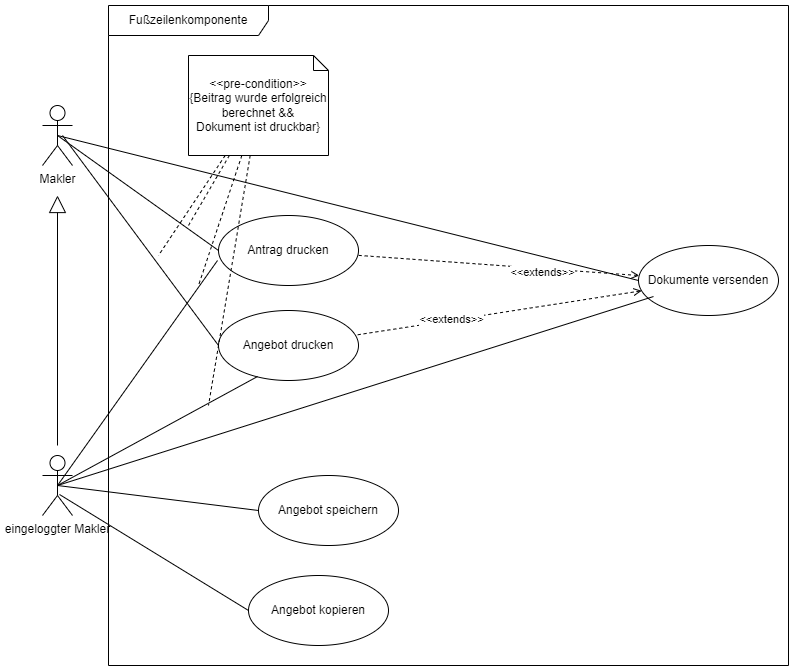
\includegraphics[width=\textwidth, height=\textheight, keepaspectratio]{anhang/usecase_footer.png}
	\caption{Anwendungsfalldiagramm der Fußzeilenkomponente}
	\label{usecasefooter}
\end{figure}
\begin{figure}[!htbp]
	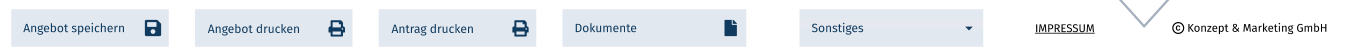
\includegraphics[width=\textwidth, height=\textheight, keepaspectratio]{anhang/mockup_footer.png}
	\caption{Mockup-Design der Fußzeile}
	\label{mockup}
\end{figure}
\begin{figure}[!htbp]
	
\includegraphics[width=\textwidth, height=\textheight, keepaspectratio]{anhang/actual_footer.png}
	\caption{Tatsächliches Design der Fußzeile}
	\label{actualfooter}
\end{figure}
\begin{figure}[!htbp]
	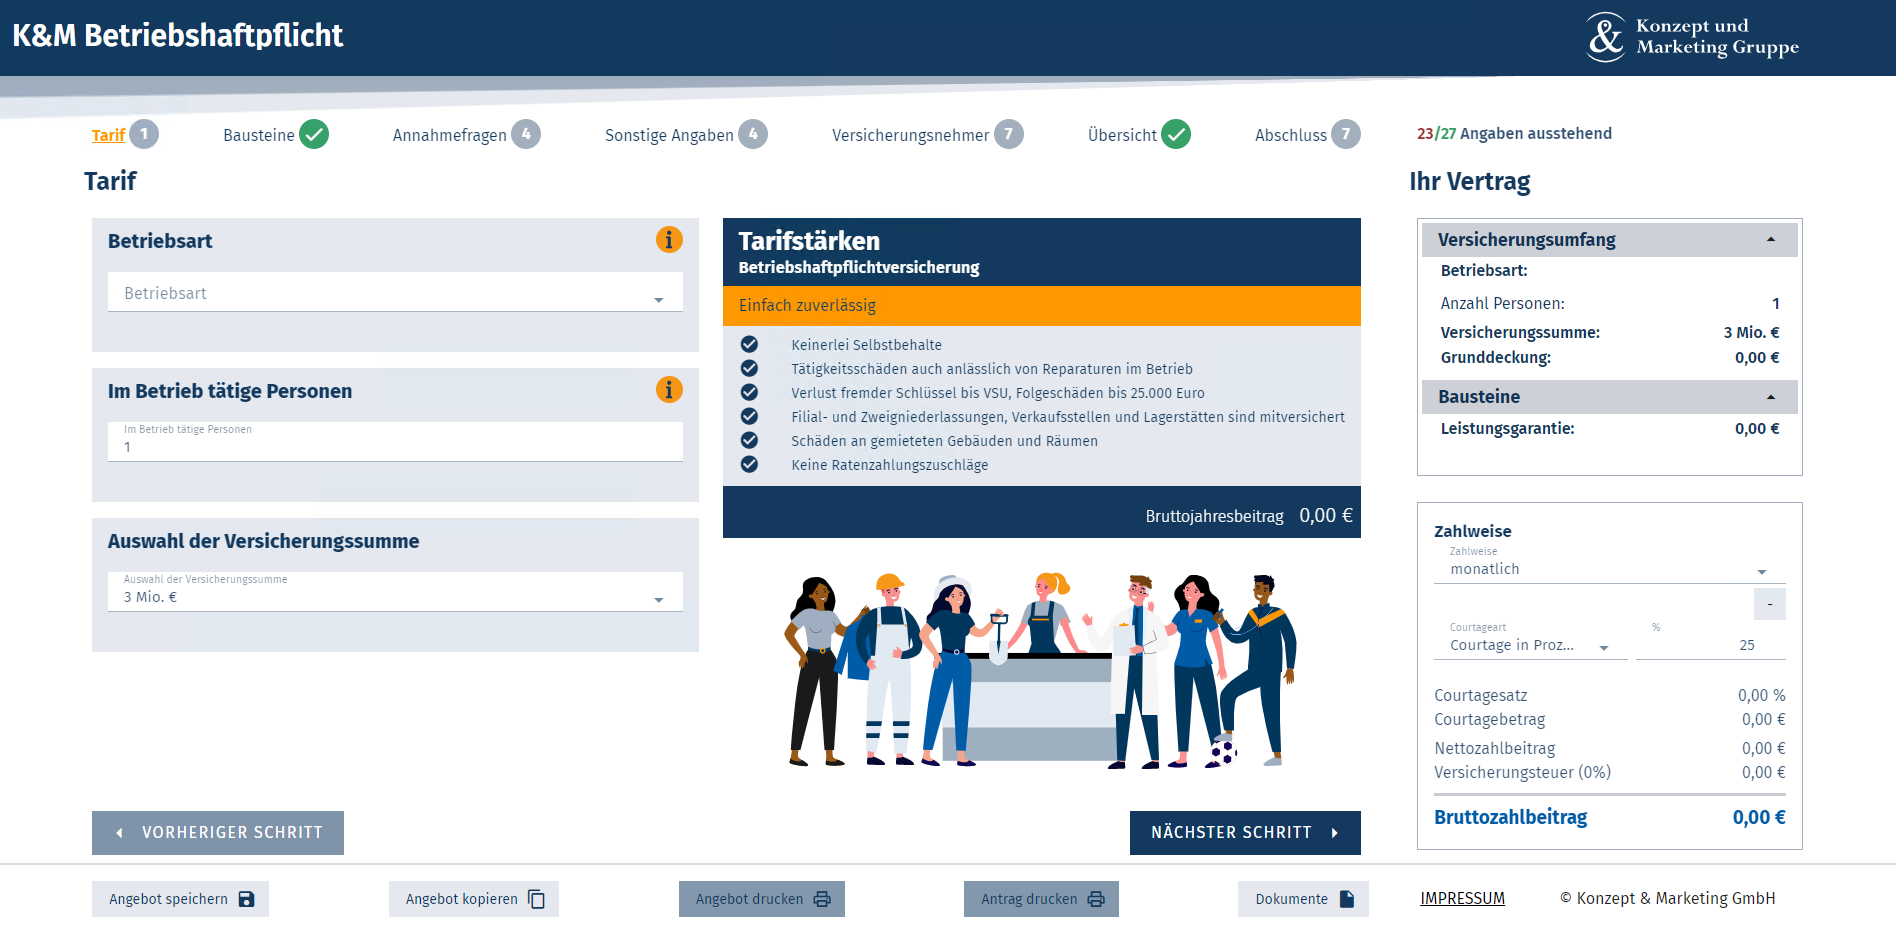
\includegraphics[width=\textwidth,  keepaspectratio]{anhang/otr.png}
	\caption{Benutzeroberfläche OTR}
	\label{otr_figure}
\end{figure}

\end{document}